%*******10********20********30********40********50********60********70********80

% For all chapters, use the newdefined chap{} instead of chapter{}
% This will make the text at the top-left of the page be the same as the chapter

\chap{Materials and Methods}\label{chap:materialsandmethods}
Lorem ipsum dolor sit amet, consectetur adipiscing elit. Pellentesque nibh metus, suscipit a scelerisque sit amet, rhoncus et lectus. Mauris eget erat rutrum, euismod massa id, maximus mauris. Nulla maximus, ex sit amet lacinia consequat, enim ante mollis dui, sit amet tincidunt massa felis id magna. Aenean gravida ante nec volutpat rutrum. Cras eget ullamcorper leo. Curabitur eu volutpat tellus. Integer nec ornare sapien. Fusce ipsum justo, interdum quis libero a, mattis tristique velit. Phasellus rhoncus lorem non ultrices luctus.
% QUI SPIEGHI IL LAVORO DI COLONNA A SAN VITO E COME FUNZIONI I CENTRI NAZIONALI DEL GLNBI
%Integra qui 7.1 \cite{GNLBI1} | 7.1.1 \cite{GNLBI2} | 7.2 \cite{GNLBI3}

\section{The population in exam}\label{sec:thepopulationinexam}
Our study sample is highly representative of the original population, since x\% ($20/32$) of the IAC adopted in Friuli-Venezia Giulia in the study period were included.
The study period spanned from 2002 to 2017. They increased year after year as graph shows.

%QUI SPIEGHI COME È FATTA LA POPOLAZIONE
%INSERISCI GRAFICO DELL'ANDAMENTO DEL NUMERO DI BAMBINI NEGLI ANNI

% US Adotpions are dropping
\vspace*{0.8cm}
\begin{figure}[h]
\centering
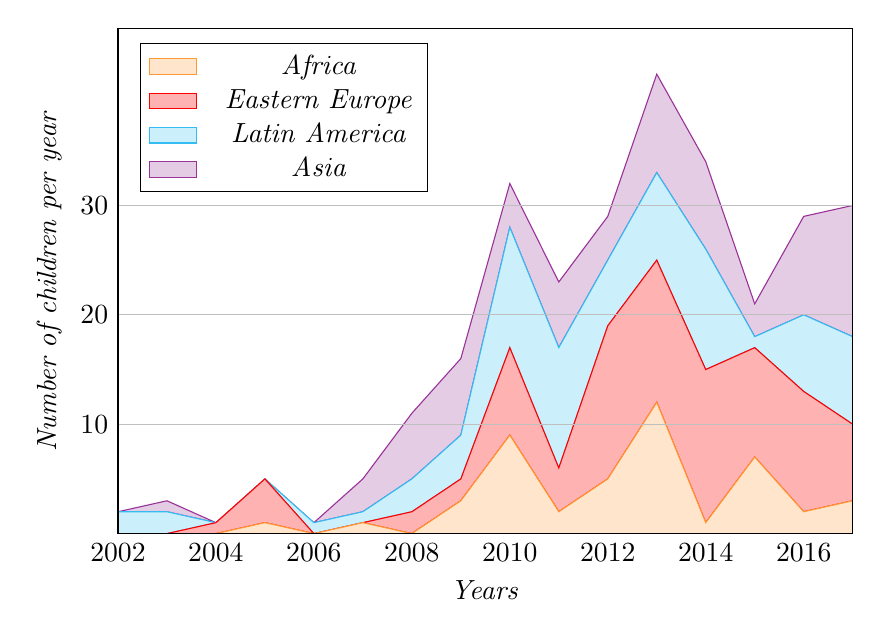
\begin{tikzpicture}
	\begin{axis}[
		stack plots=y,
		area style,
		enlarge x limits=false,
		enlarge y limits=upper,
		width=0.9\textwidth,
		height=8cm,
		xlabel = \textit{Years},
         ylabel = \textit{Number of children per year},
         ytick = {10, 20, 30},
         ytick style={draw=none},
         xtick style={draw=none},
         x tick label style={/pgf/number format/.cd,%
          scaled x ticks = false,
          set thousands separator={},
          fixed},
         y tick label style={/pgf/number format/.cd,%
          scaled y ticks = false,
          set thousands separator={},
          fixed},
         ymajorgrids=true,
         legend style={column sep=8pt},
         legend pos = north west]
    \addplot [draw={orange!80!white},fill={orange!20!white}] coordinates %Africa
		{(2002, 0) (2003, 0) (2004, 0) (2005, 1) (2006, 0) (2007,1 ) (2008, 0) (2009, 3) (2010, 9) (2011, 2) (2012, 5) (2013, 12) (2014, 1) (2015, 7) (2016, 2) (2017, 3)} 
		\closedcycle;
		\label{figdata:africa}
	\addplot coordinates % Eastern Europe
		{(2002, 0) (2003, 0) (2004, 1) (2005, 4) (2006, 0) (2007, 0) (2008, 2) (2009, 2) (2010, 8) (2011, 4) (2012, 14) (2013, 13) (2014, 14) (2015, 10) (2016, 11) (2017, 7)} 
		\closedcycle;
		\label{figdata:easterneurope}
	\addplot [draw={cyan!80!white},fill={cyan!20!white}] coordinates % Latin America
		{(2002, 2) (2003, 2) (2004, 0) (2005, 0) (2006, 1) (2007, 1) (2008, 3) (2009, 4) (2010, 11) (2011, 11) (2012, 6) (2013, 8) (2014, 11) (2015, 1) (2016, 7) (2017, 8)} 
		\closedcycle;
		\label{figdata:latinamerica}
		\addplot [draw={violet!80!white},fill={violet!20!white}] coordinates  % Asia
		{(2002, 0) (2003, 1) (2004, 0) (2005, 0) (2006, 0) (2007, 3) (2008, 6) (2009, 7) (2010, 4) (2011, 6) (2012, 4) (2013, 9) (2014, 8) (2015, 3) (2016, 9) (2017, 12)} 
		\closedcycle;
		\label{figdata:asia}
		\legend{\textit{Africa},\textit{Eastern Europe},\textit{Latin America},\textit{Asia}}
	\end{axis}
\end{tikzpicture}
\caption{Our population distribution - Total of children visited via the screening protocol, stratified by geographic area of origin}
\label{fig:populationperyear}
\end{figure}

\subsection{Inclusion and exclusion citeria}\label{sub:inclusionandexclusionciteria}
Lorem ipsum dolor sit amet, consectetur adipiscing elit. Pellentesque nibh metus, suscipit a scelerisque sit amet, rhoncus et lectus. Mauris eget erat rutrum, euismod massa id, maximus mauris. Nulla maximus, ex sit amet lacinia consequat, enim ante mollis dui, sit amet tincidunt massa felis id magna. Aenean gravida ante nec volutpat rutrum. Cras eget ullamcorper leo. Curabitur eu volutpat tellus. Integer nec ornare sapien. Fusce ipsum justo, interdum quis libero a, mattis tristique velit. Phasellus rhoncus lorem non ultrices luctus.

%QUI CHI È DENTRO E CHI È FUORI E PERCHÉ. ELENCO PUNTATO?

\section{The data set}\label{sec:dataset}
Lorem ipsum dolor sit amet, consectetur adipiscing elit. Pellentesque nibh metus, suscipit a scelerisque sit amet, rhoncus et lectus. Mauris eget erat rutrum, euismod massa id, maximus mauris. Nulla maximus, ex sit amet lacinia consequat, enim ante mollis dui, sit amet tincidunt massa felis id magna. Aenean gravida ante nec volutpat rutrum. Cras eget ullamcorper leo. Curabitur eu volutpat tellus. Integer nec ornare sapien. Fusce ipsum justo, interdum quis libero a, mattis tristique velit. Phasellus rhoncus lorem non ultrices luctus.

%QUI SPIEGHI COME SONO STATI RACCOLTI I DATI DA COLONNA
% RIFERISCI A tab:columnparameter O INSERISCILA QUI

\section{Data set elaboration}\label{sec:datasetelaboration}
Lorem ipsum dolor sit amet, consectetur adipiscing elit. Pellentesque nibh metus, suscipit a scelerisque sit amet, rhoncus et lectus. Mauris eget erat rutrum, euismod massa id, maximus mauris. Nulla maximus, ex sit amet lacinia consequat, enim ante mollis dui, sit amet tincidunt massa felis id magna. Aenean gravida ante nec volutpat rutrum. Cras eget ullamcorper leo. Curabitur eu volutpat tellus. Integer nec ornare sapien. Fusce ipsum justo, interdum quis libero a, mattis tristique velit. Phasellus rhoncus lorem non ultrices luctus.

%QUI SPIEGHI COME E' FATTO IL DB

\subsection{VBA expressions}\label{sub:vbaexpressions}
Lorem ipsum dolor sit amet, consectetur adipiscing elit. Pellentesque nibh metus, suscipit a scelerisque sit amet, rhoncus et lectus. Mauris eget erat rutrum, euismod massa id, maximus mauris. Nulla maximus, ex sit amet lacinia consequat, enim ante mollis dui, sit amet tincidunt massa felis id magna. Aenean gravida ante nec volutpat rutrum. Cras eget ullamcorper leo. Curabitur eu volutpat tellus. Integer nec ornare sapien. Fusce ipsum justo, interdum quis libero a, mattis tristique velit. Phasellus rhoncus lorem non ultrices luctus.

All VBA expression can be found in Appendix \ref{chap:appendixvbaexpressions} at page \pageref{chap:appendixvbaexpressions}.

%INSERT REF TO SECTION OF CODE HERE

\subsection{Cut-off values}\label{sub:cutoffvalues}
Lorem ipsum dolor sit amet, consectetur adipiscing elit. Pellentesque nibh metus, suscipit a scelerisque sit amet, rhoncus et lectus. Mauris eget erat rutrum, euismod massa id, maximus mauris. Nulla maximus, ex sit amet lacinia consequat, enim ante mollis dui, sit amet tincidunt massa felis id magna. Aenean gravida ante nec volutpat rutrum. Cras eget ullamcorper leo. Curabitur eu volutpat tellus. Integer nec ornare sapien. Fusce ipsum justo, interdum quis libero a, mattis tristique velit. Phasellus rhoncus lorem non ultrices luctus.

%INSERT WHERE THEY COME FROM
%INSERT TABLES HERE

\subsubsection{Haemoglobin}\label{sub:haemoglobin}
This was a little prick. 

%INSERT ELENCO PUNTATO DA COSA DIPENDE
%INSERT TABLE HERE

\subsubsection{MCV}\label{sub:mcv}
This was ANOTHER little prick. 

%INSERT ELENCO PUNTATO DA COSA DIPENDE
%INSERT TABLE HERE

\subsubsection{Circulating Iron}\label{sub:iron}
This was easy.

%INSERT WHAT IT MEANS
%INSERT TABLE HERE

\subsubsection{Vitamin D}\label{sub:vitaminD}
Vitamin D is healthy. 25OH...

%INSERT WHAT IT MEANS
%https://en.wikipedia.org/wiki/Calcifediol
%INSERT WHY THIS IS BEEN DOSED
%INSERT TABLE HERE

\subsection{Parasites grouping}\label{sub:parasites}
%QUI SI PARLA DI PERCHE LI HAI DIVISI IN DUE GRUPPI E COME (SUL FATTO CHE FOSSERO ANEMIZZANTI O MENO) E POI VEDIAMO I RISULTATI
% IN \cite{GNLBIexp} C'è una tabella con cui comparare i risultati!!

\section{Statistical Analyses}\label{sec:statisticalanalyses}
Le analisi descrittive sono state condotte utilizzando frequenze e percentuali per variabili categoriche, e medie e deviazioni standard o mediane e intervalli interquartili per variabili continue, con una preferenza per queste ultime a causa del campione esiguo di dati che non consente di verificare la normalità dei dati.

La differenza nei valori di variabili continue in diversi gruppi è stata valutata con test non parametrici di Mann-Whitney o Kruskal-Wallis a seconda che i gruppi da confrontare fossero due o più di due. Per lo studio di associazione tra due variabili dicotomiche, o tra una variabile dicotomica e una categoriale ordinata abbiamo utilizzato il test esatto di Fisher a due code. Per studiare se un esito dicotomico fosse associato a una o più variabili indipendenti abbiamo utilizzato la regressione logistica.
Per studiare la relazione tra due variabili continue, abbiamo preferito utilizzare la correlazione per ranghi di Spearman.

Per tutte le analisi abbiamo usato il software Stata/IC 14.2 (StataCorp LLC, College Station, USA).


%QUI SPIEGHI QUALI ELABORAZIONI SONO STATE USATE